% !TeX root = ../../../main.tex

All the methods outlined in \cref{sec:mhou/estimates} are suitable to provide
an uncertainty estimate on the theoretical prediction of an observable value.
With more or less extra assumptions, the exact definition of this uncertainty
actually corresponds to \textit{probability distribution} over the value
predicted.

During a \pdf fit, probability distributions are already involved, but they
only appears on the experimental data side.
So, the normal workflow consist to compare a probability distribution coming
from data with the individual value provided by theoretical predictions, and
minimize the $\chi^2$ distance.
%
This is already not the whole story, since the \nnpdf methodology accounts also
for the \pdf distribution, that generates a distribution for theory predictions
through the theory map of \fktab{}s (cf. \cref{ch:pine}).
%
But \nnpdf, with its \mc approach, accounts for this distribution one \pdf
replica at a time, reducing the problem to minimize the $\chi^2$ distance, with
the probability distributions (assumed to be Gaussian) only on experimental
side once more.

However, the introduction of theory uncertainties generates once more a
distribution for the theoretical prediction values, by appointing the
distribution not on the \pdf, but on the theory map itself.
%
In order to deal with these distributions, another approach is required.

This problem has been faced for the first time by the \acrlong{nnpdf} in
\cite{NNPDF:2019ubu}.
%
The strategy adopted is described in section 2 of the reference, and basically
consists in assuming a Gaussian distribution for the theory predictions (for a
single \pdf candidate), finding that this will modify to usual probability
distribution for the shifts between theory predictions and experimental data
only in the covariance matrix.
%
Essentially, the probability distribution is still a Gaussian, as it is in
absence of theory uncertainties, but the full covariance matrix turns out to be
simply the sum of the experimental and theoretical covariance matrices.

\begin{figure}
	\centering
	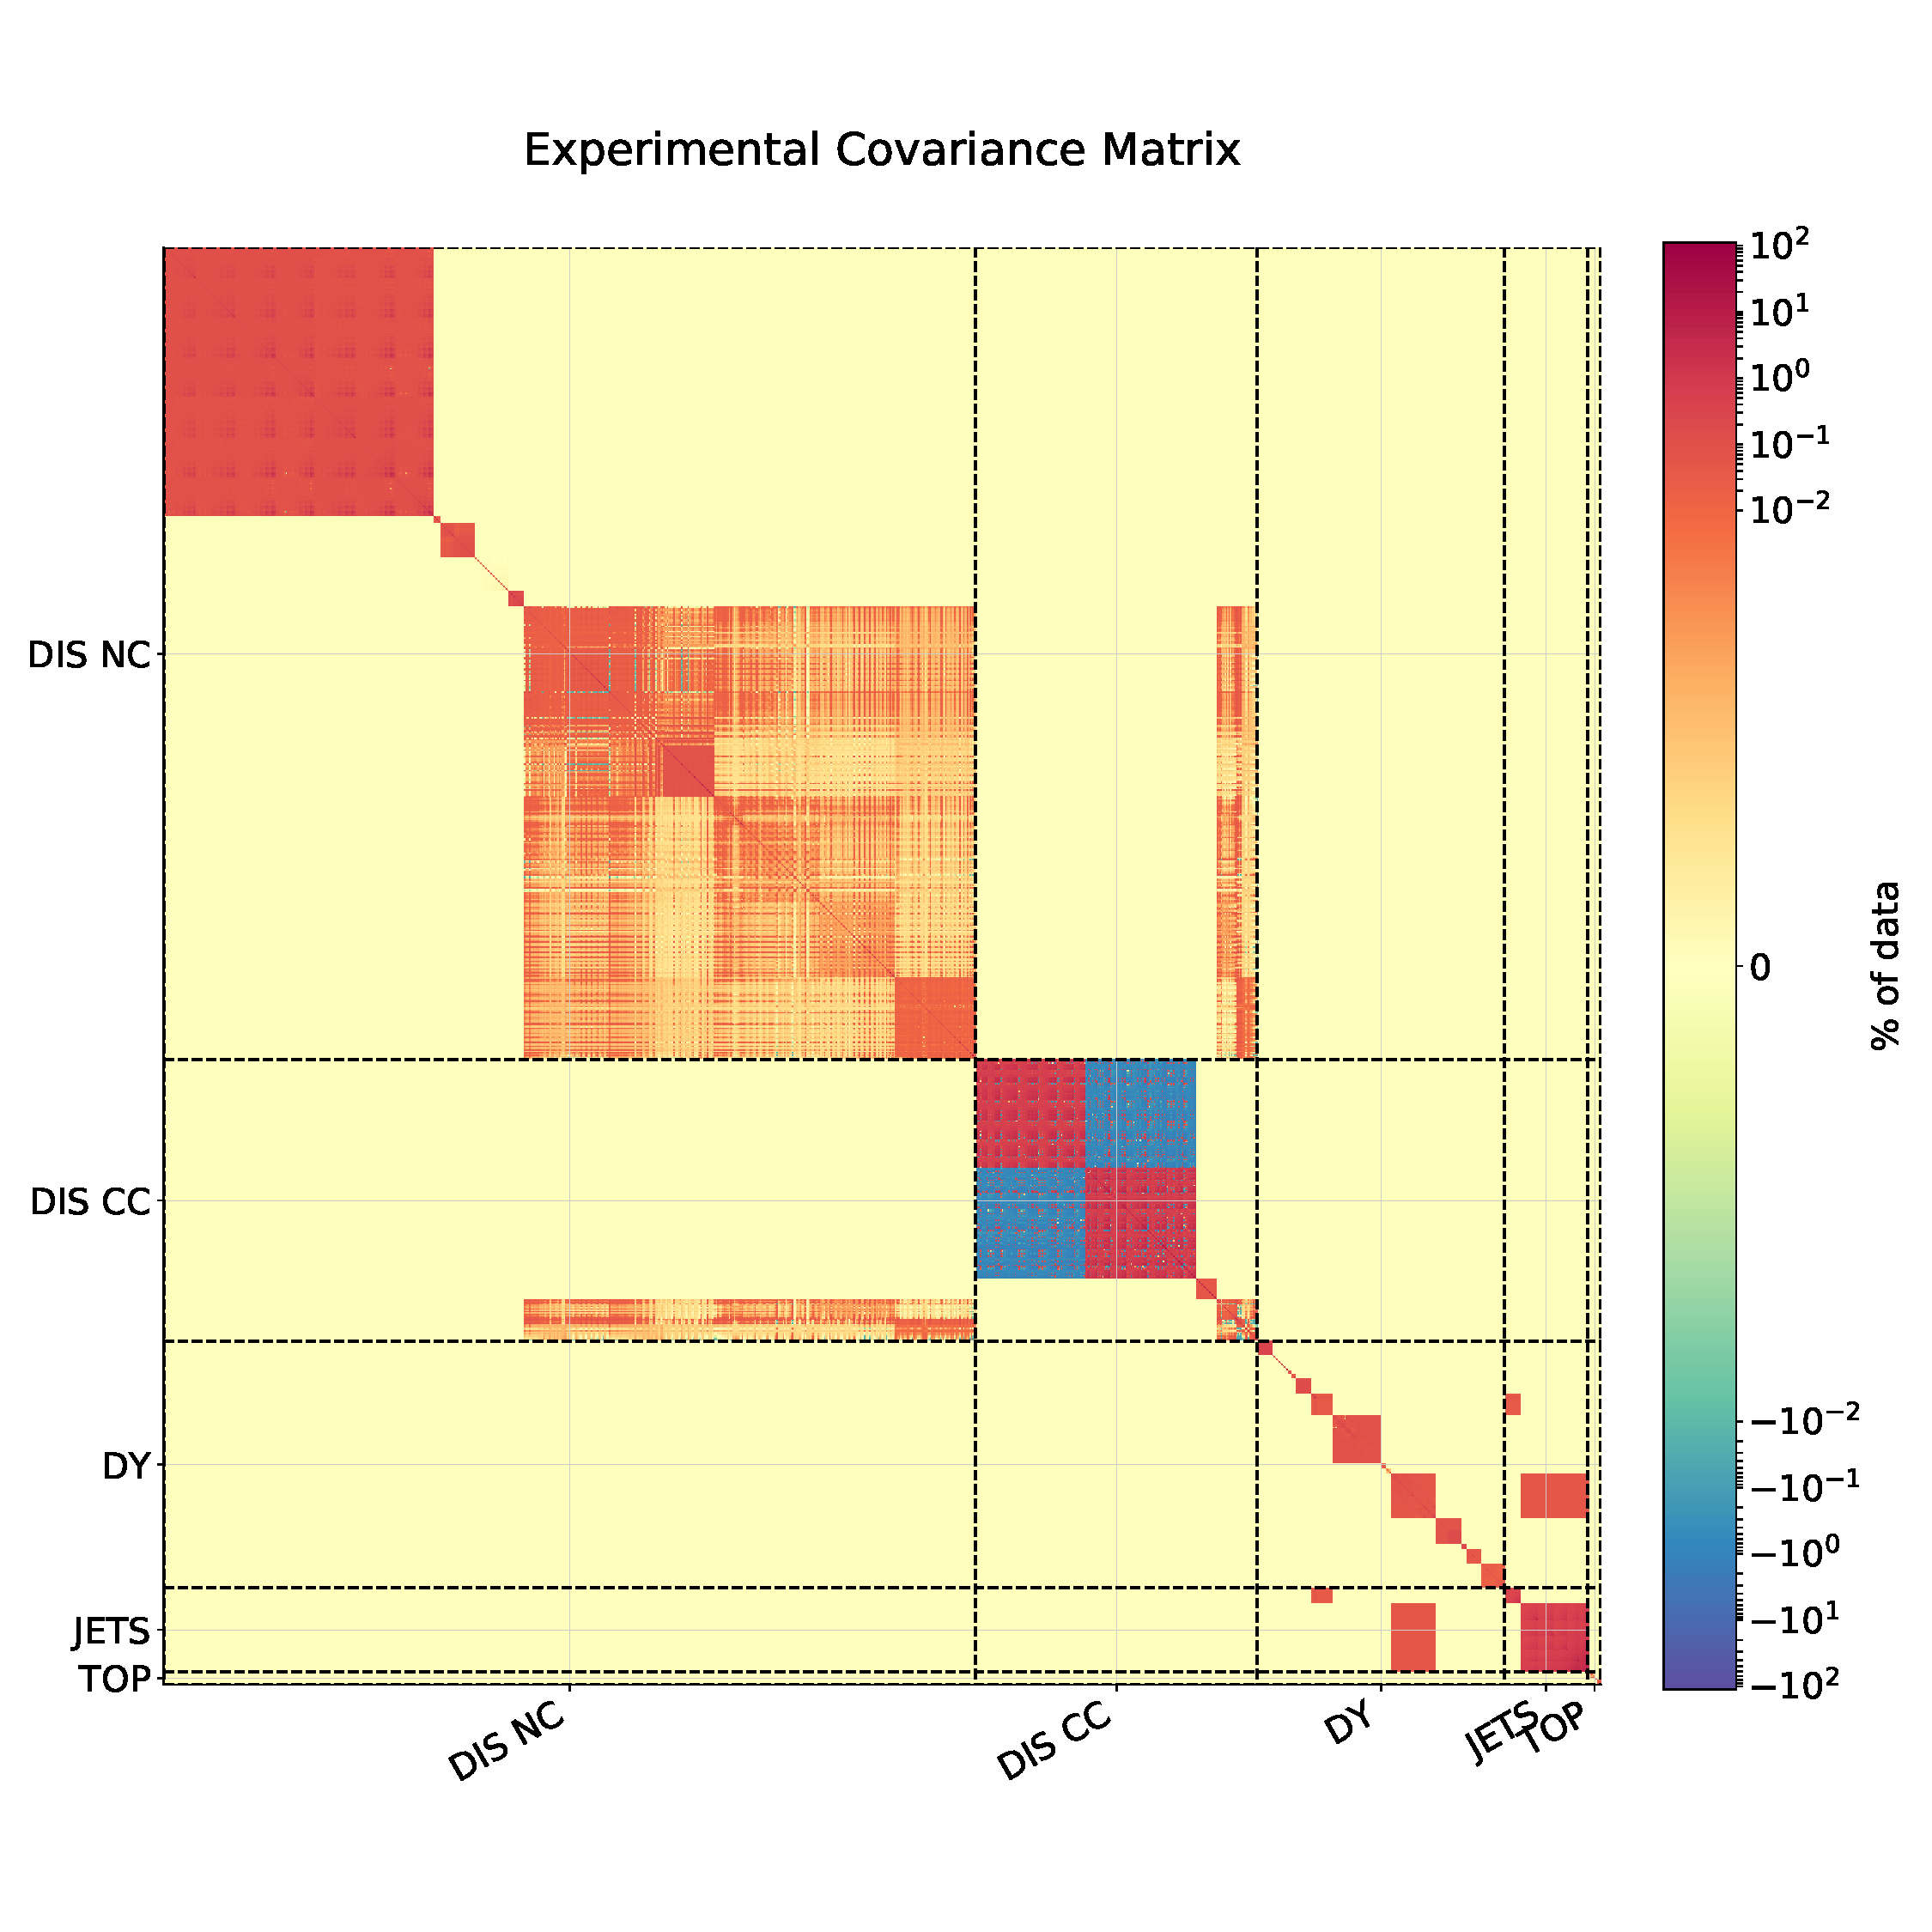
\includegraphics[width=0.49\hsize]{ch-mhou/exp_covmat}
	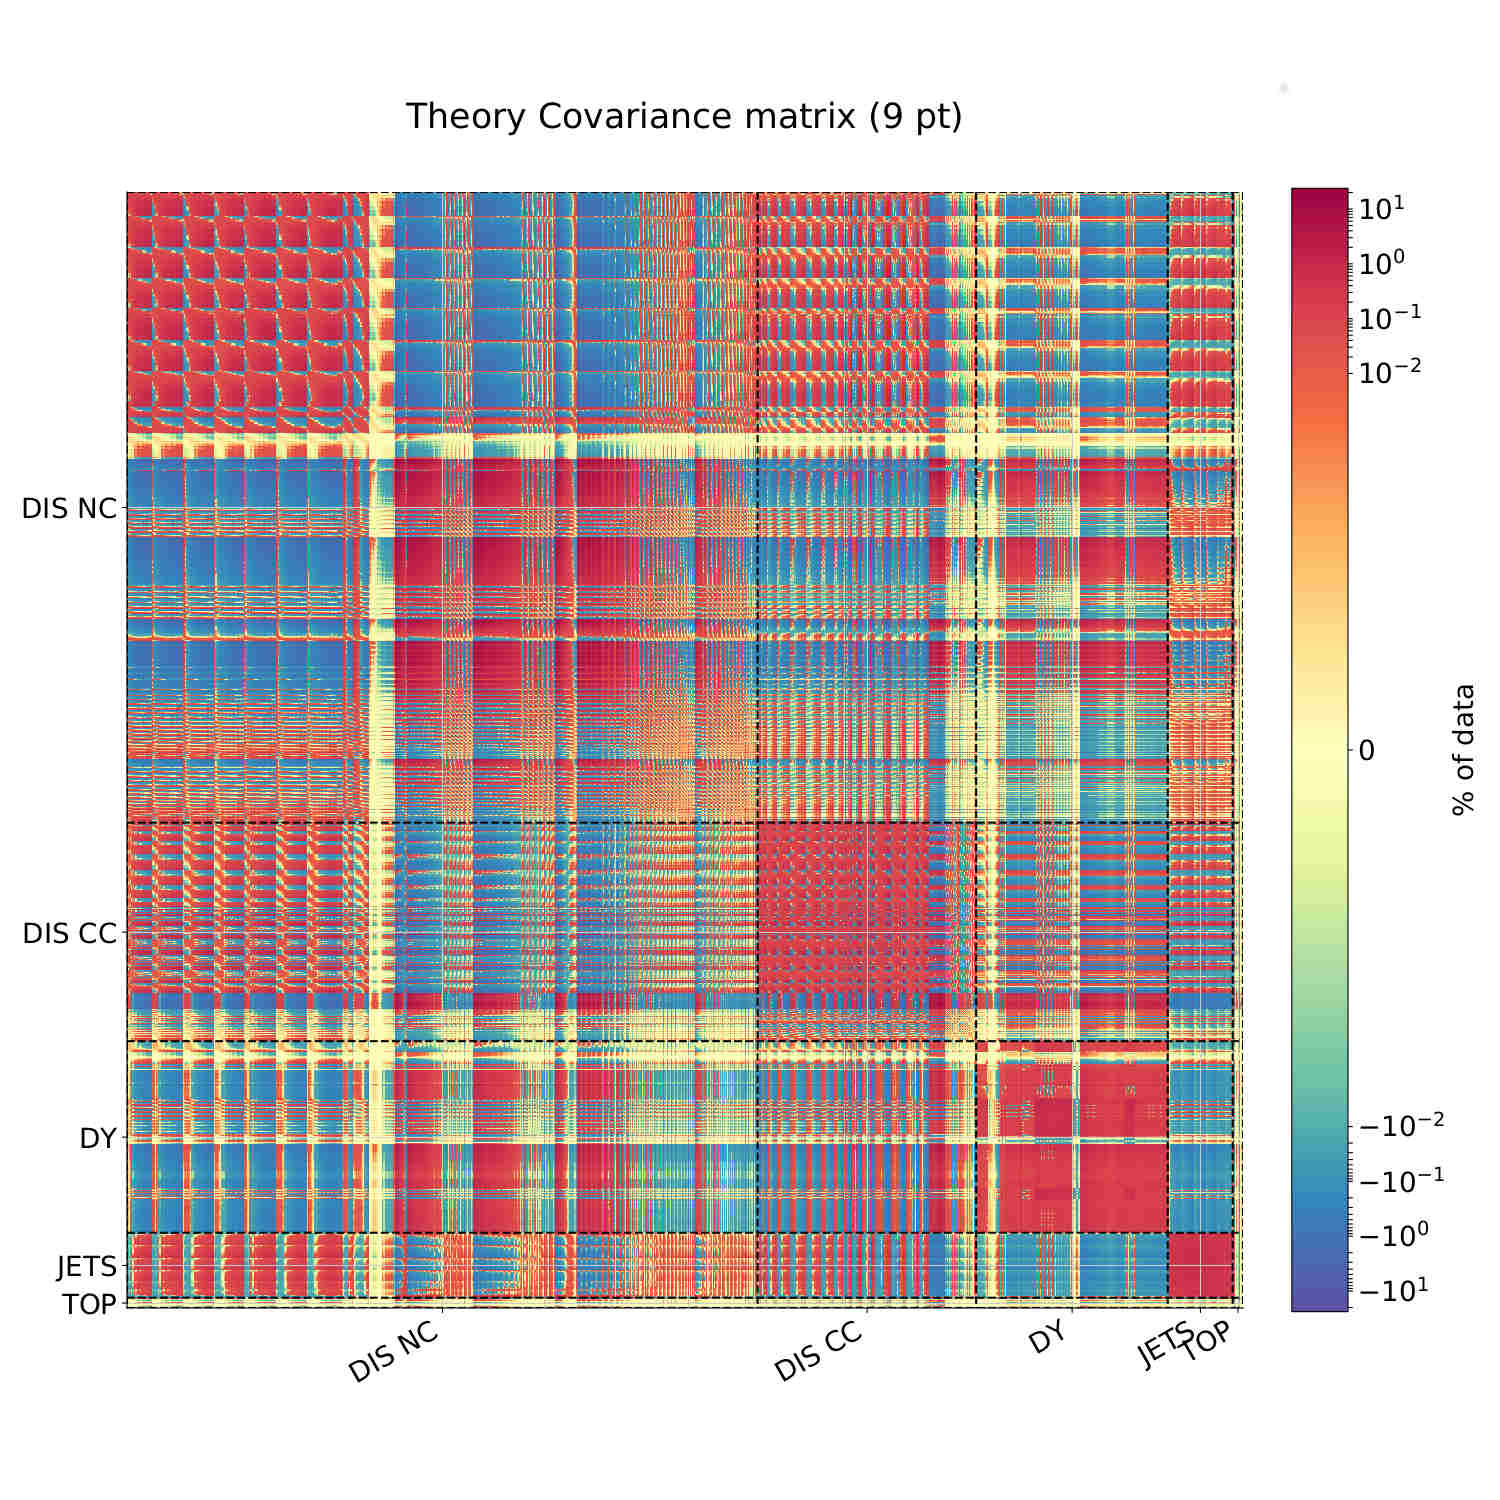
\includegraphics[width=0.49\hsize]{ch-mhou/th_covmat_9pt}
	\caption{
		Comparison between the experimental covariance matrix and the
		theoretical one, generated by the 9 point prescriptions, both
		normalized to central values.
	}
	\label{fig:mhou/covmats}
\end{figure}

In \cref{fig:mhou/covmats} the two matrices are shown for the \nnpdfr{3.1}
dataset, using colors to represent the entries as percentages of the central
values\footnote{
  These plots, and the following ones in this section, are all taken from
  \cite{NNPDF:2019ubu} and used to illustrate the readers the concept
  discussed.
  Cf.\ the reference for further details about the plots themselves.
}.
The theoretical one is computed using the 9 points prescription, that is
explained, together with the other point prescriptions in
\cref{sec:mhou/prescriptions}.
%
The sum of the two matrices, i.e.\ the actual covariance matrix used in the
\nnpdfr[3.1th+]{3.1th} fit, is shown in \cref{fig:mhou/combined-covmat}.

\begin{figure}
	\centering
	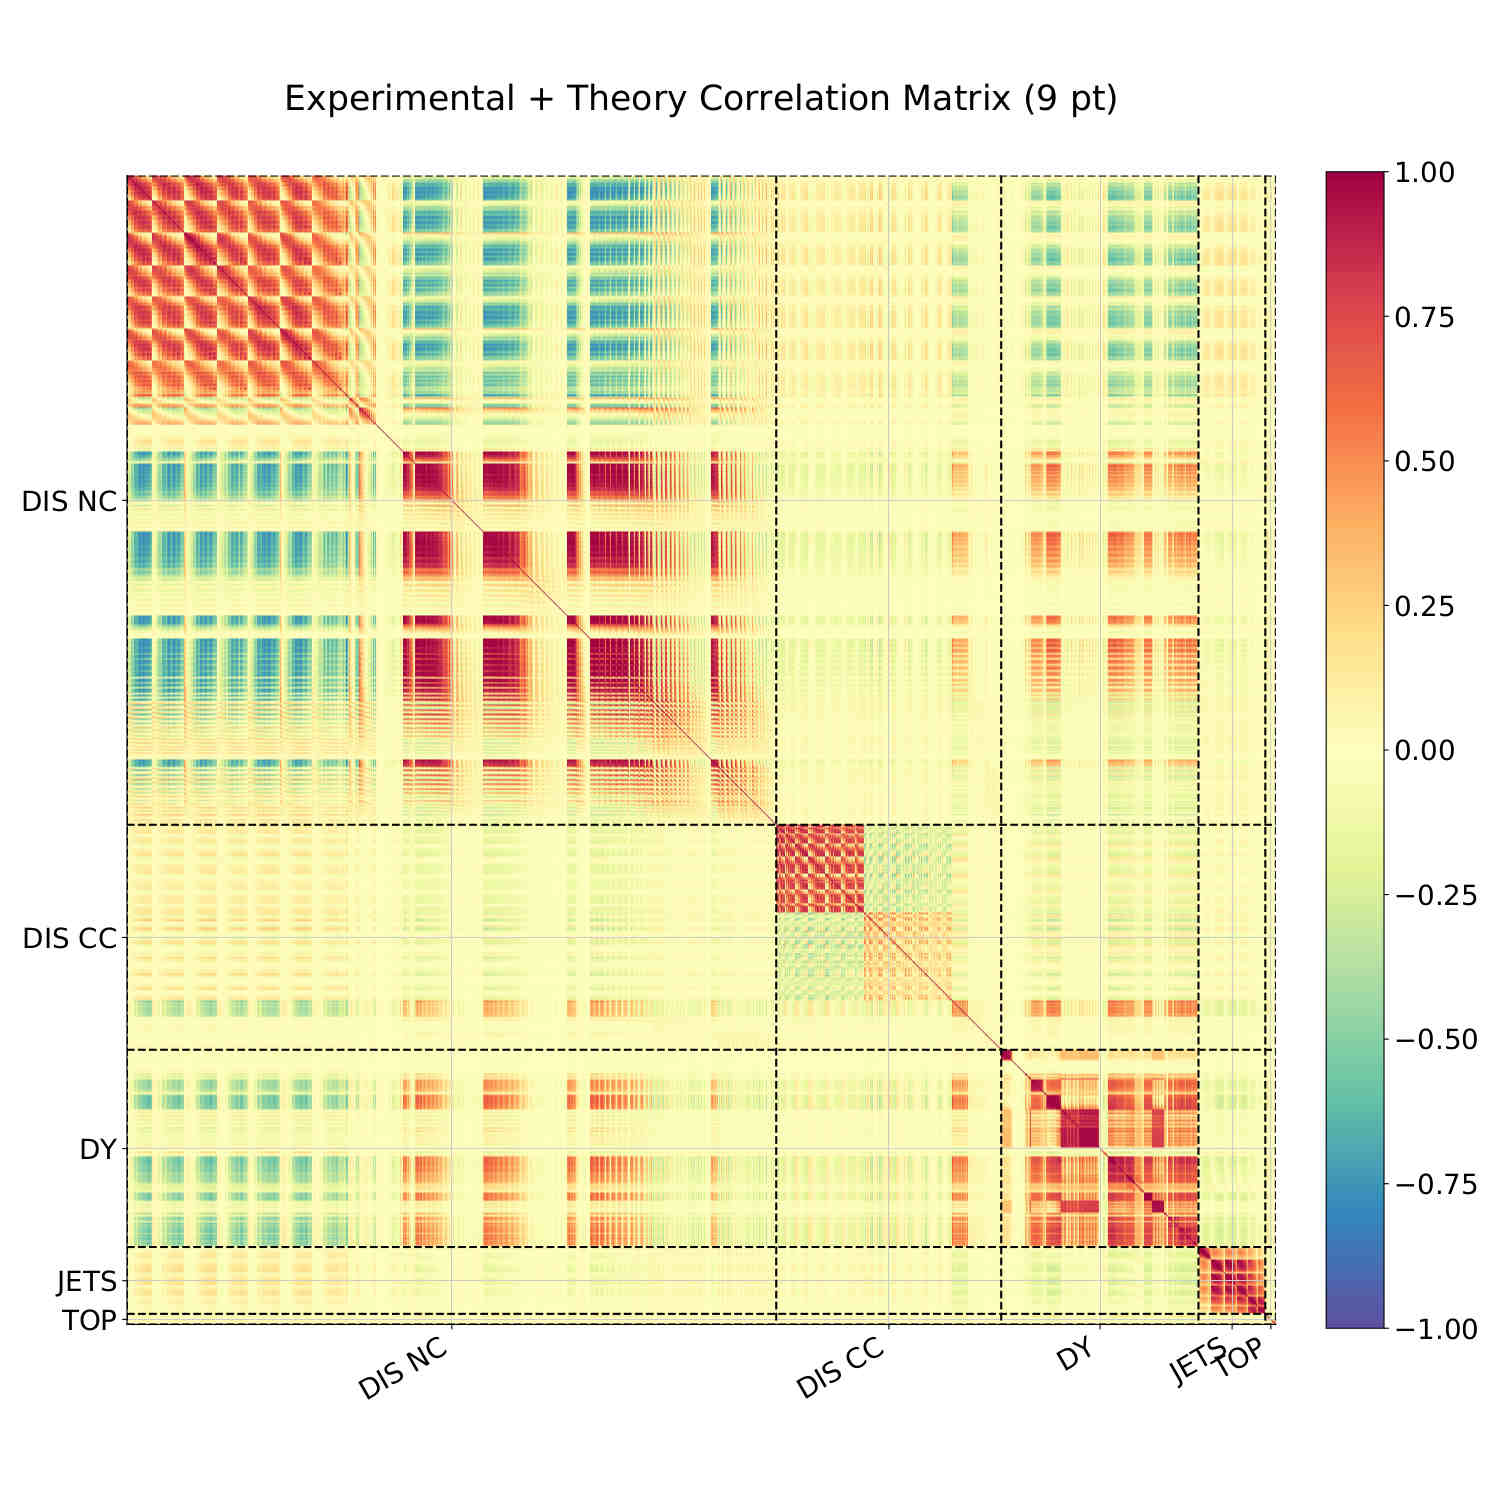
\includegraphics[width=0.7\hsize]{ch-mhou/expth_corrmat_9pt}
	\caption{
		Combined covariance matrix (experimental plus theoretical), the actual
		one used in the \nnpdfr[3.1th+]{3.1th} fit.
	}
	\label{fig:mhou/combined-covmat}
\end{figure}

In \cite{NNPDF:2019ubu} the \mhou study stops at \nlo, but since \nnlo central
values are already available (used in the baseline for \nnpdfr{3.1}) it is possible 
to compare the size of the estimated uncertainties (variances of individual
observables, i.e.\ diagonal entries of the combined covariance matrix) to the
actual shift between the \nlo and \nnlo central values for the central value of
\nnpdfr{3.1} \pdf set.
%
This comparison plot is shown in \cref{fig:mhou/scvar-shifts}, still using the
same 9 points prescription adopted for the theory covariance matrices used in
previous figures.
%
It is important to note that the \nnlo in the \pdf is not included in the very
same way of \nlo, apart for \dis values (still the most part in the
\nnpdfr{3.1} dataset).
Indeed, in order to produce \nnlo values for a generic \pdf candidate a \nlo
interpolation grid (cf. \cref{ch:pine}) is \textit{upgraded} to an approximate
\nnlo one by means of $K$-factors, i.e.\ under the hypothesis that the only
difference between the two orders is only the global normalization, that is
obtained by the ratio of predictions computed with an already available \pdf
set (usually the former release of \nnpdf itself, making the process
iterative).

\begin{figure}
	\centering
	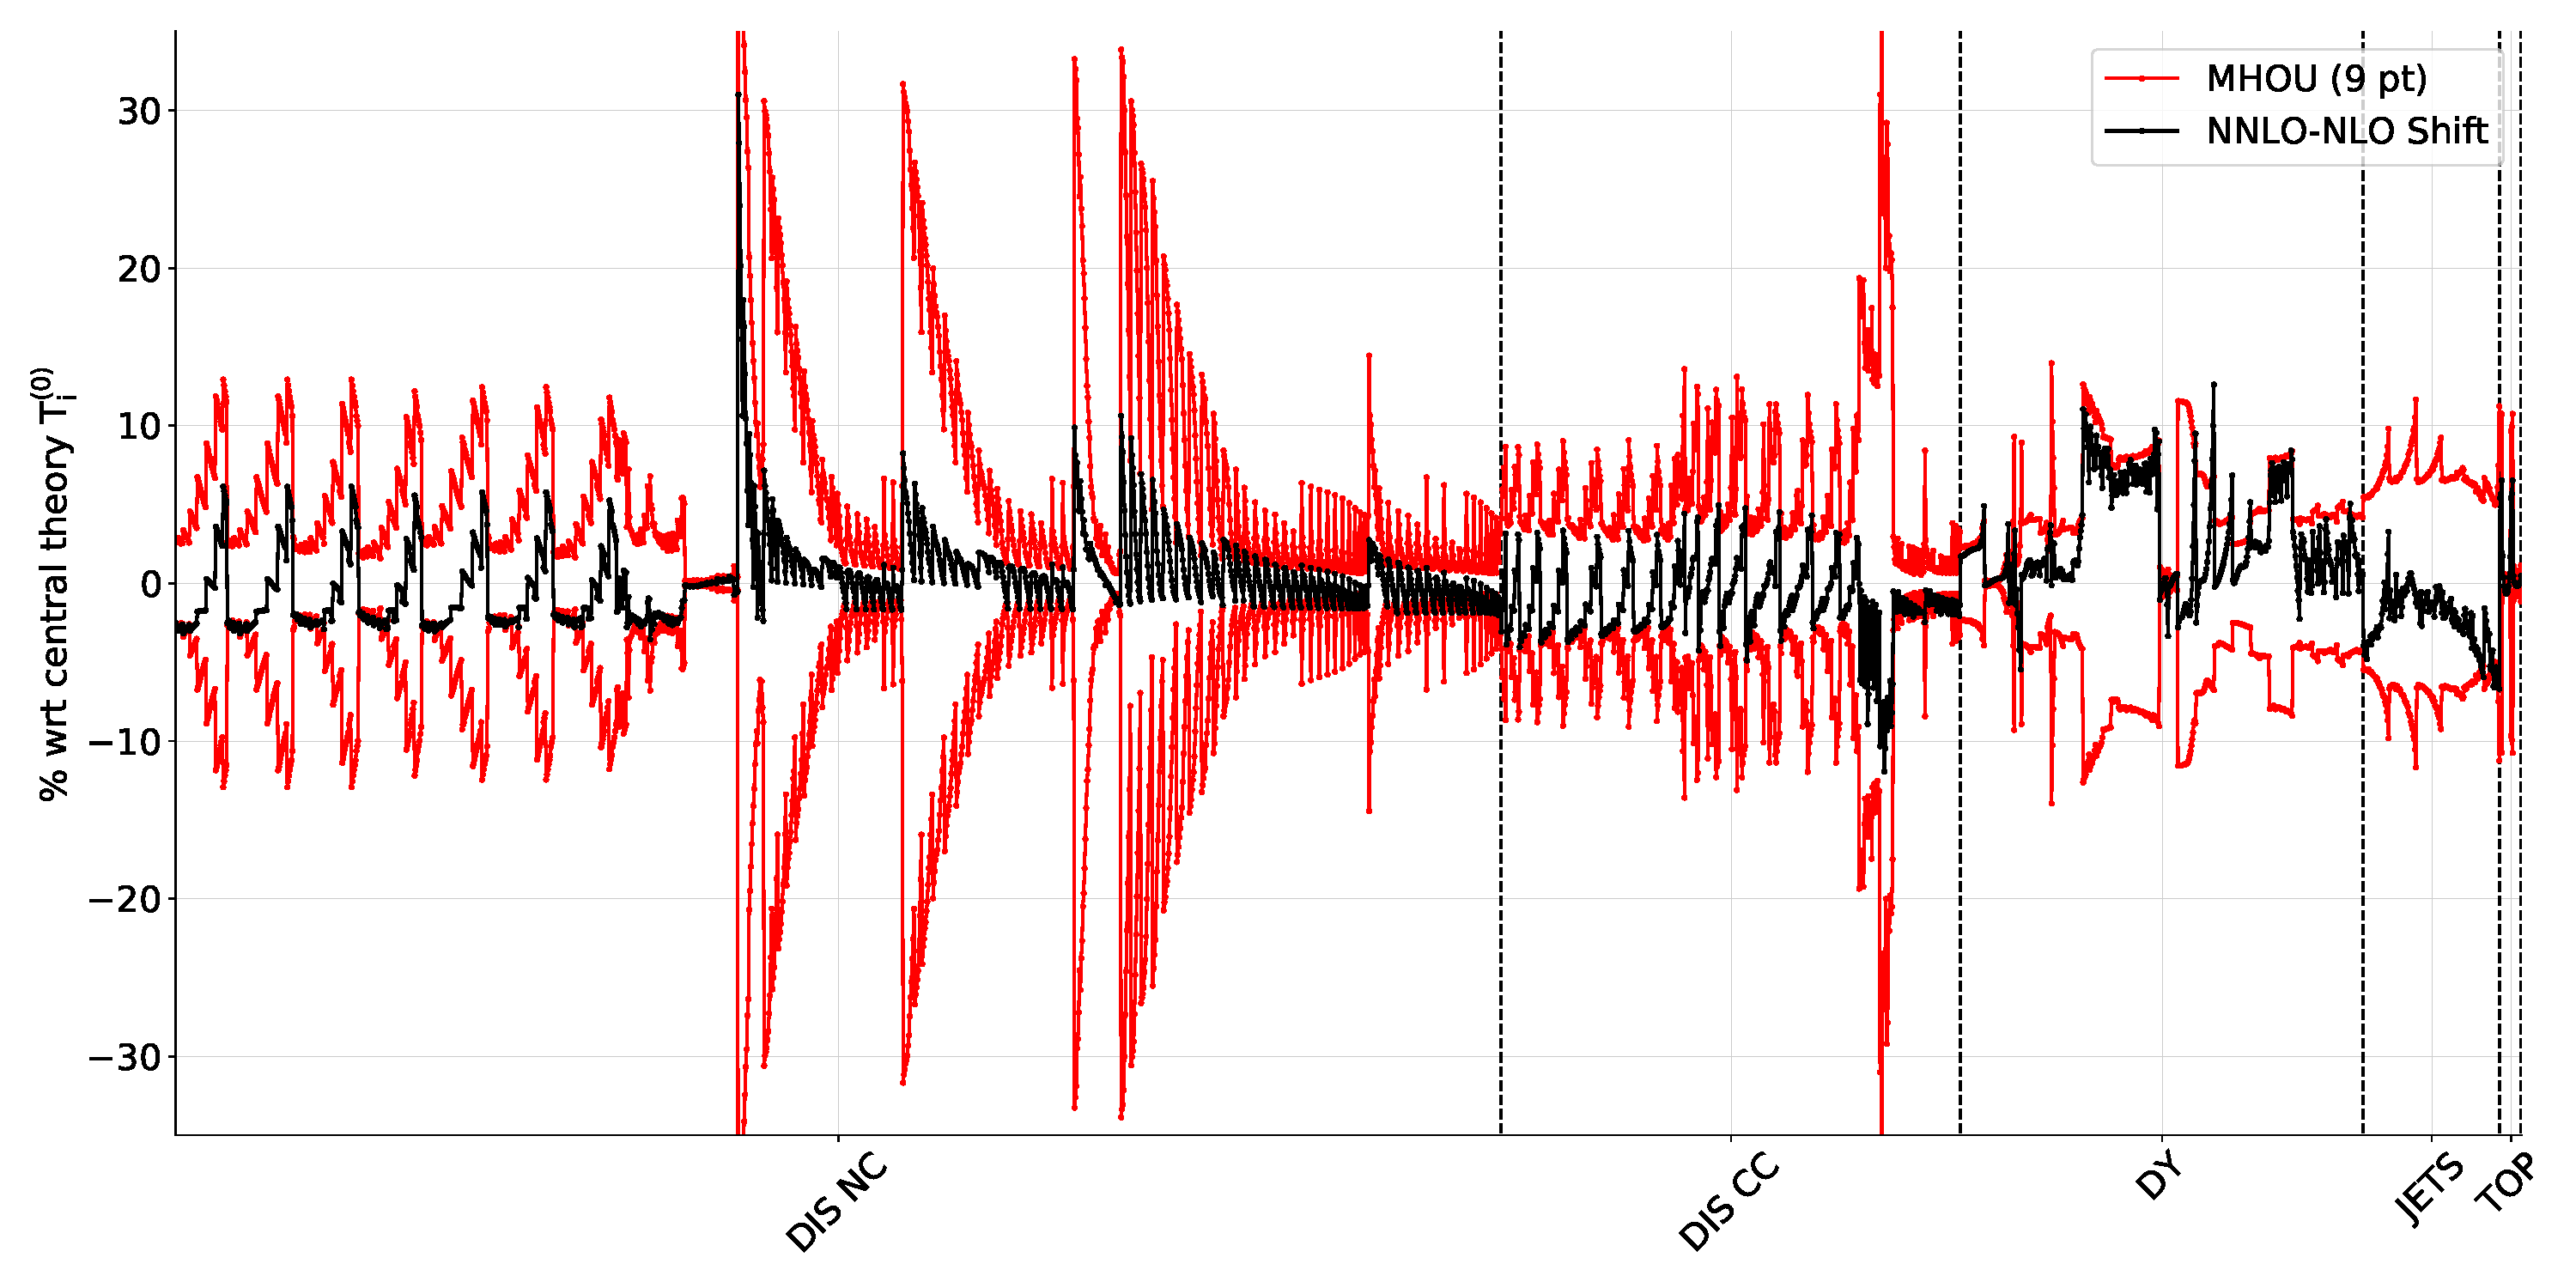
\includegraphics[width=\hsize]{ch-mhou/shift_diag_cov_comparison_9pt_global}
	\caption{
		The diagonal uncertainties $\sigma_i$ (red) symmetrized about zero,
		compared to the shift $\delta_i$ for each data-point (black).
		Values are shown as percentage of the central theory prediction
	}
	\label{fig:mhou/scvar-shifts}
\end{figure}

The final result for a fit including the combined covariance matrix is shown in
\cref{fig:mhou/3.1th}.
%
This set is the \nnpdfr[3.1th+]{3.1th} release, and it is available on the
\nnpdf website and as an \lhapdf website, on the respective website,
\url{https://lhapdf.hepforge.org/pdfsets}.

\begin{figure}
	\centering
	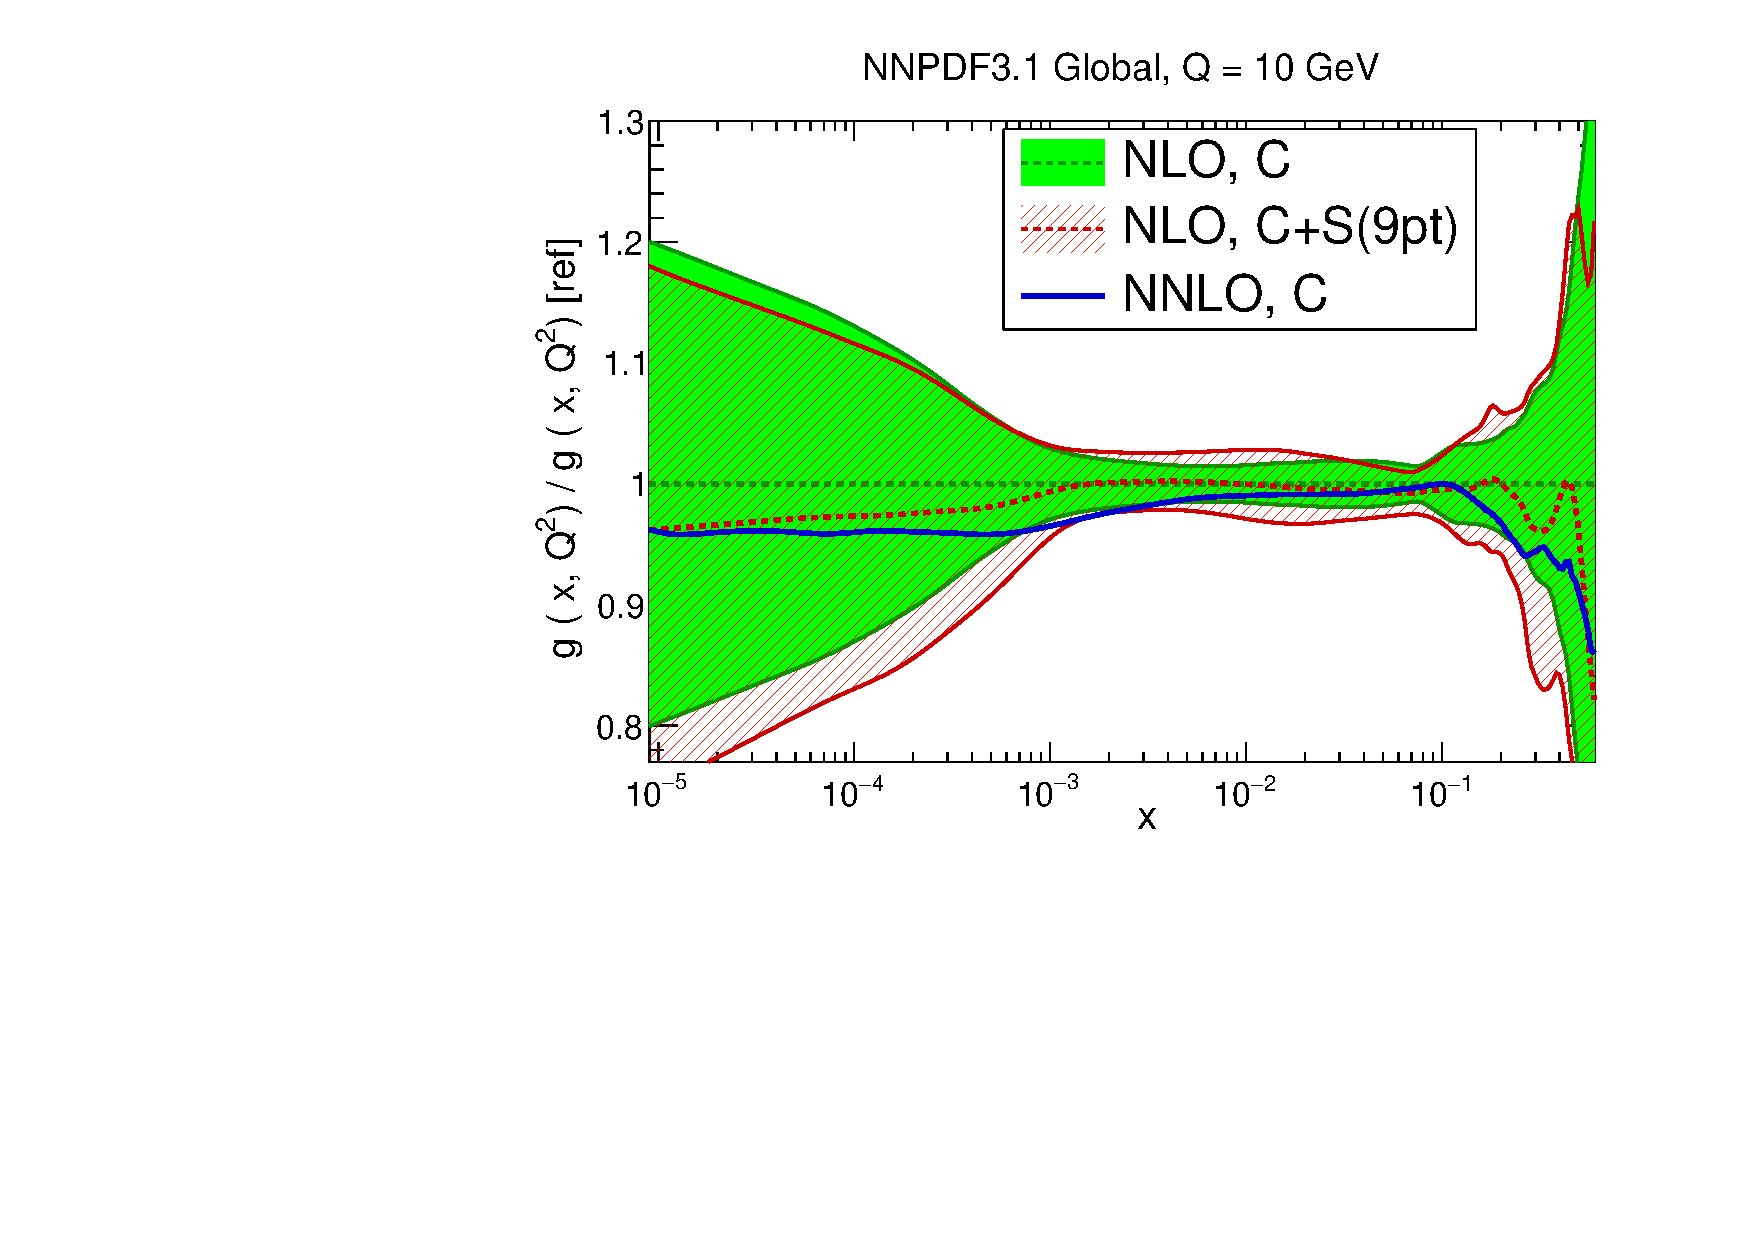
\includegraphics[width=0.49\hsize]{ch-mhou/xg-Global-NLO-CovMatTH-EXP-vsTH}
	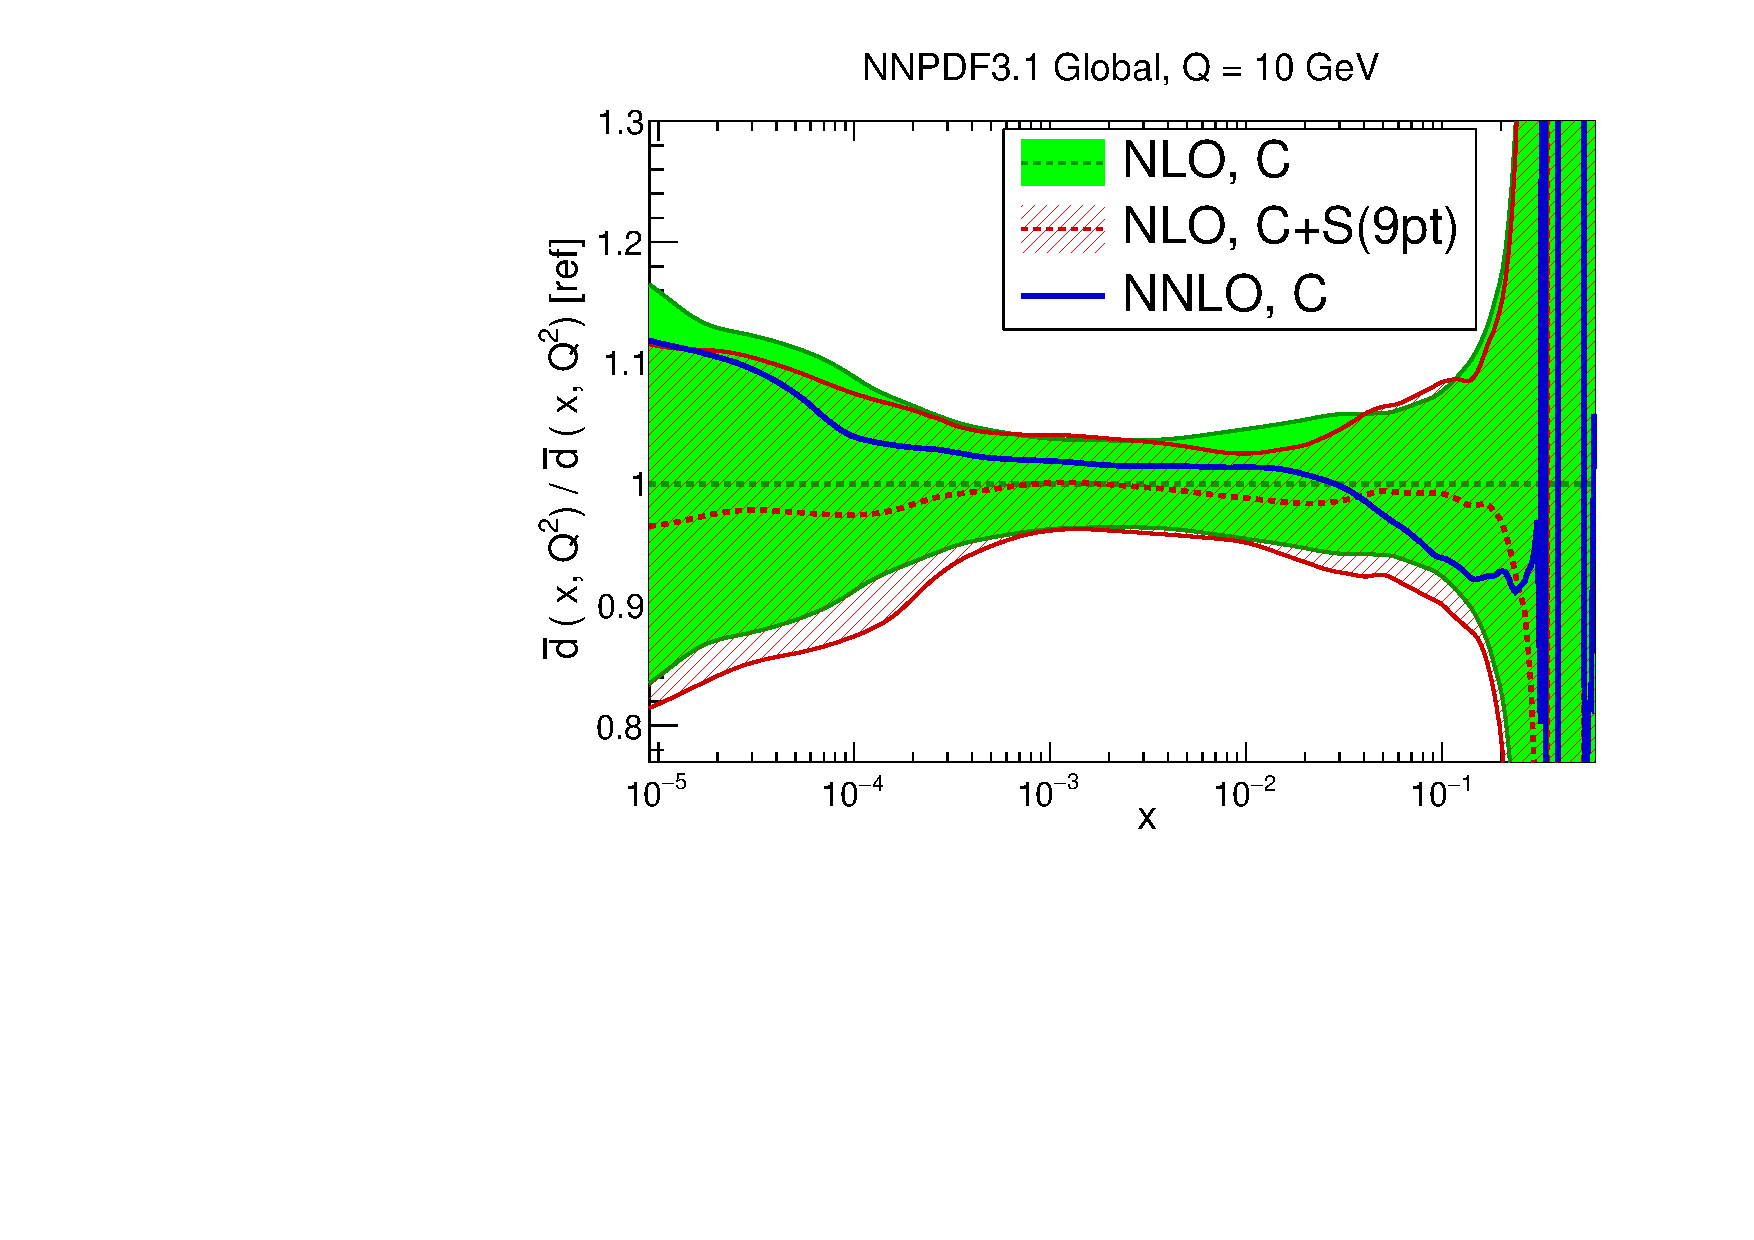
\includegraphics[width=0.49\hsize]{ch-mhou/xdbar-Global-NLO-CovMatTH-EXP-vsTH}
	\caption{
		\nnpdfr[3.1th+]{3.1th} \nlo sets, gluon and anti-down distributions at
		$\SI{10}{\giga\electronvolt}$, the first \pdf determination to include
		\mhou estimates in the fit.
	}
	\label{fig:mhou/3.1th}
\end{figure}

It is important to remark that the combined covariance matrix has to be used in
all the places in which the experimental covariance matrix was used, i.e.\ all
the places in which the distribution enters.
%
Indeed, the effect of the theory distribution, under the assumptions in
\cite{NNPDF:2019ubu} discussed above, is to modify the covariance matrix in the
distribution, and so in all its instances in the \pdf fit.
%
In particular, the distribution (and so the covariance matrix) is used in two
places:
\begin{enumerate}[label=\roman*.]
  \item the definition of the $\chi^2$ to be minimized
  \item the generation of pseudo-data, part of the \nnpdf methodology (better
    explained in \cref{ch:gp}, or in \nnpdf literature, such as
    \cite{Ball:2008by})
\end{enumerate}
%
The effect of using the combined covariance in a single instance, while keeping
the experimental one for the other (as in the baseline), is shown in
\cref{fig:mhou/3.1th-tests}.

\begin{figure}
	\centering
	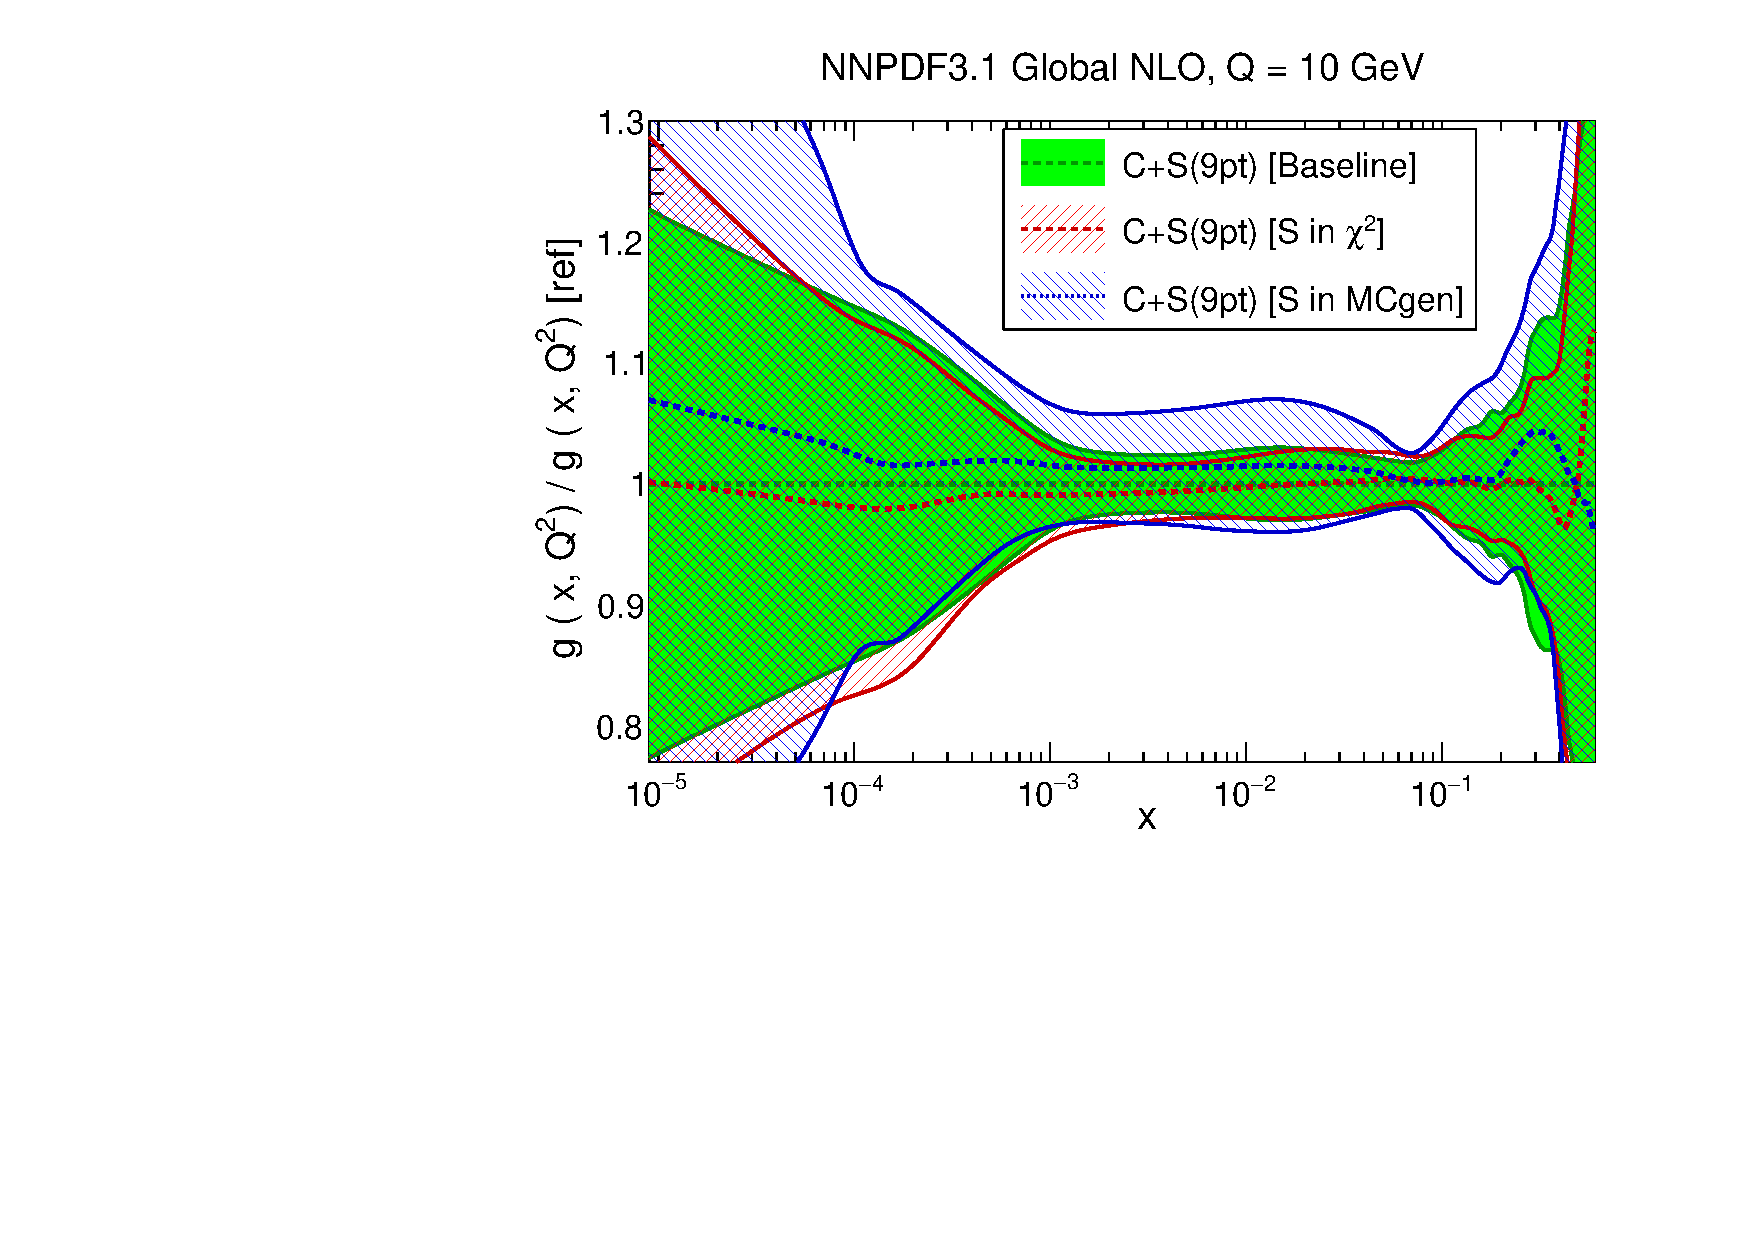
\includegraphics[width=0.49\hsize]{ch-mhou/xg-Global-NLO-CovMatTH-tests}
	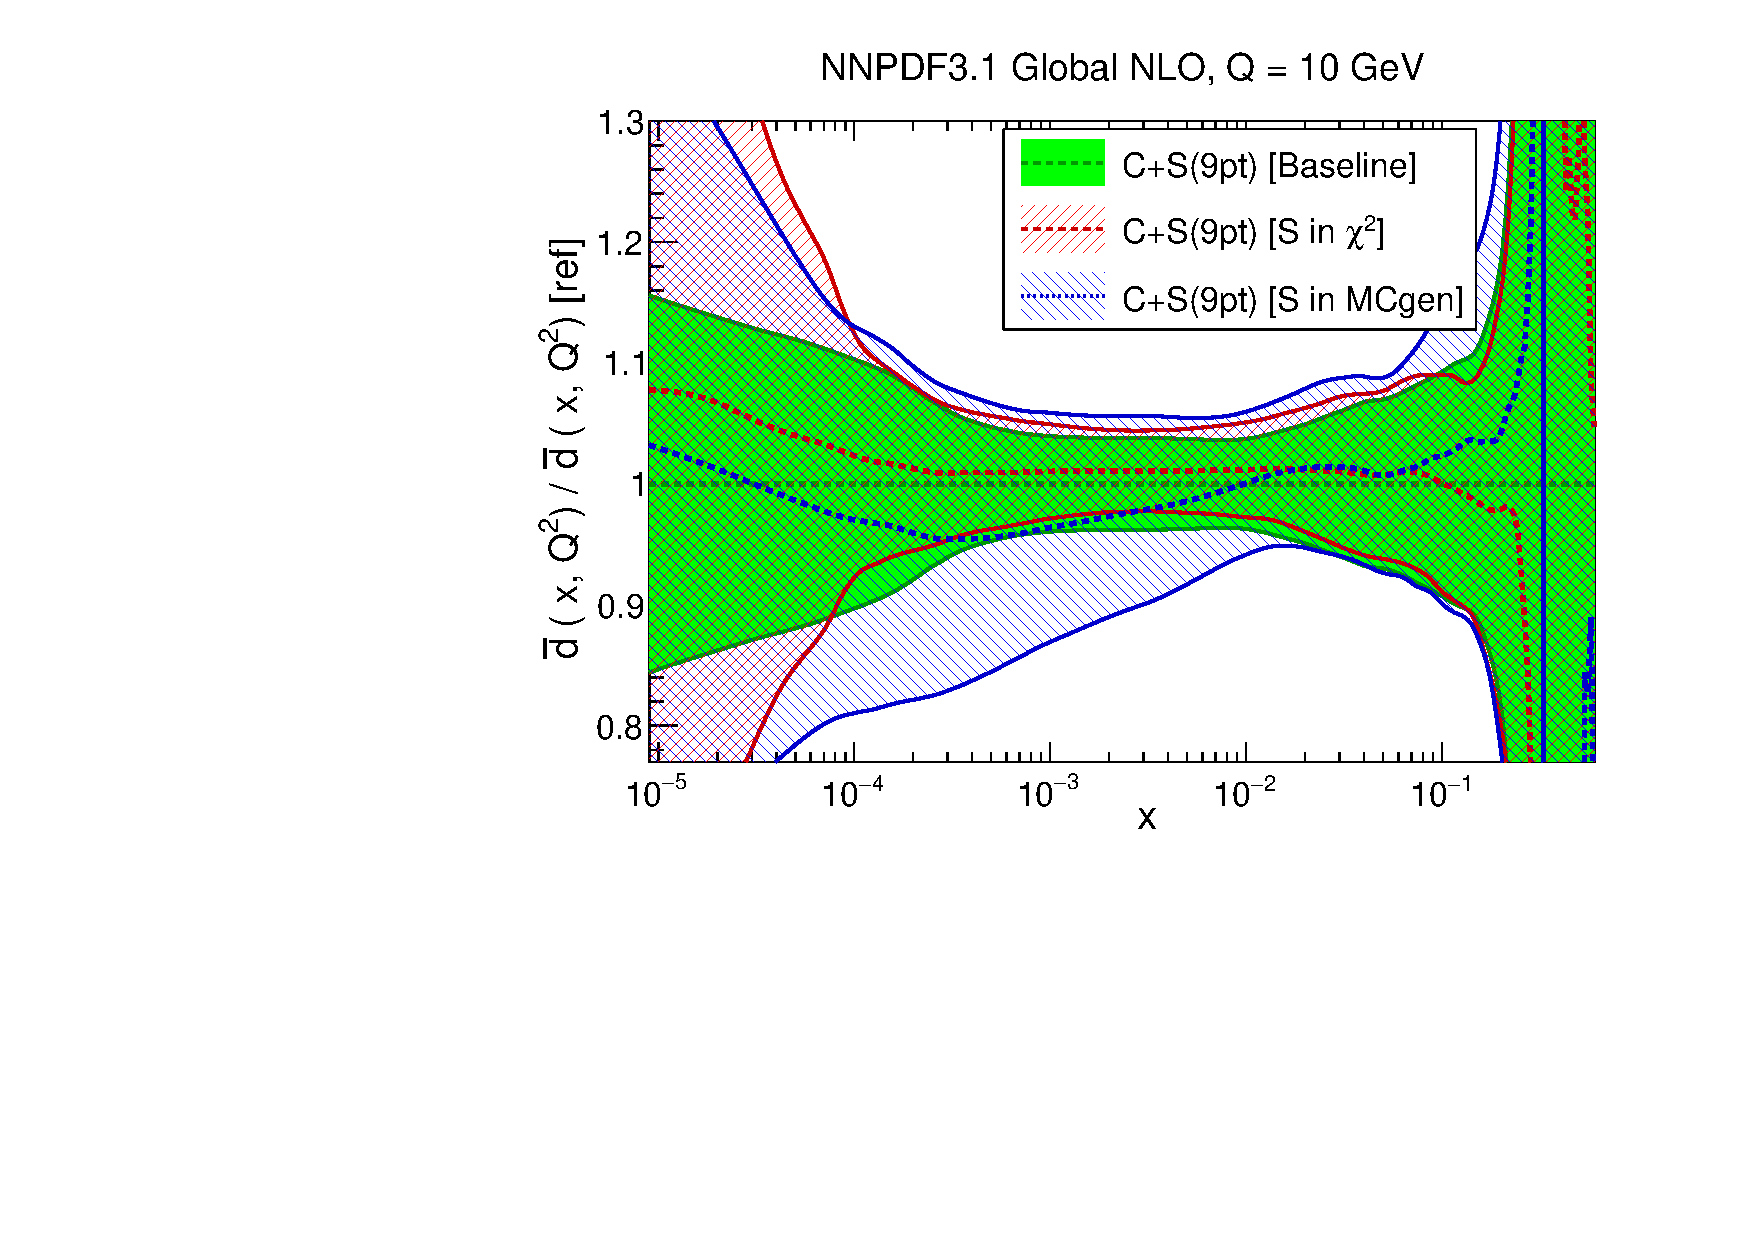
\includegraphics[width=0.49\hsize]{ch-mhou/xdbar-Global-NLO-CovMatTH-tests}
	\caption{
		Gluon and anti-down distributions comparison, in which it is shown the
		effect of using the theory covariance matrix in the $\chi^2$ or in the
		pseudo-data generation only.
	}
	\label{fig:mhou/3.1th-tests}
\end{figure}
